\chapter{Learning the basics}
Hazelcast is a datagrid implementation for the JVM, so any language that runs on the JVM can make use of Hazelcast. Hazelcast makes it easy to create scalable and high available applications.

\section{Installing Hazelcast}

First you need to make sure that Java 5 or higher is installed on your machine. If not installed, it can be downloaded from the Oracle site:
http://java.com/en/download/index.jsp. After you ensured that Java is installed, Hazelcast can be downloaded from http://www.hazelcast.com/downloads.jsp. There are 2 versions:

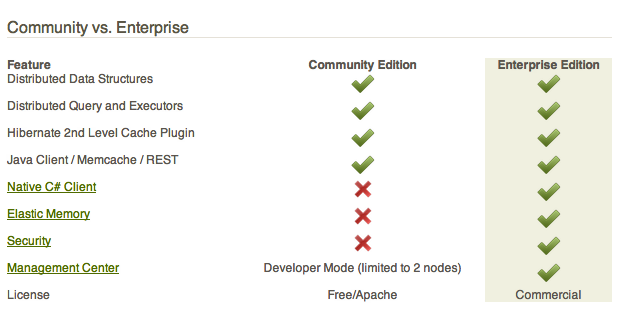
\includegraphics[scale=0.60]{hazelcast-editions.png}

For our purposes of this book we'll rely on the community edition. If your project relies on Maven, there is no need to install Hazelcast. Setting the dependencies is enough, see next chapter.

\section{Hazelcast and Maven}

Hazelcast is very easy to include in your Maven project without needing to install Hazelcast at all.  Hazelcast can be found in the standard maven repositories, so no need to added additional repositories to your Maven project. To include Hazelcast in your project, just add the following to your pom.xml:

\begin{verbatim}
<dependencies>	
   ...
   <dependency>
      <groupId>com.hazelcast</groupId>
      <artifactId>hazelcast</artifactId>
      <version>2.1.2</version>
   </dependency>

</dependencies>
\end{verbatim}	

Make sure that you check the Hazelcast website to make use of the most recent version. 

After this dependency is added, Maven will automatically downloaded the dependencies needed. The lack of needing to install Hazelcast is something I really like because it saves up quite a lot of time, so we can spend that time doing more useful things.

\section{Configuring Hazelcast}

Programmatic, Spring, xml-configuration file.

\section{}


\section{Configure logging}

